\documentclass{beamer}
% Beamer automatically loads amsmath, amssymb, amsthm, hyperref, graphicx

\usetheme[progressbar=frametitle]{metropolis}
% metropolis automatically loads tikz

\usepackage{bookman}
\renewcommand{\familydefault}{\rmdefault}

\title{Presentations}
\author{Tony Mendes}
\institute{Cal Poly San Luis Obispo}
\date{}

\begin{document}


\begin{frame}
\titlepage
\end{frame}


\begin{frame}[fragile] % fragile is needed to use \verb

  \frametitle{How to use the Beamer class}
  
  \begin{enumerate}
      \item Use \verb~beamer~ in \verb~\documentclass~, not \verb~article~. \\[5ex]
      \item Create slides with code in a \verb~frame~ environment. 
  \end{enumerate}

\end{frame}


\begin{frame}[fragile]
\frametitle{Tips for good design}

\begin{enumerate}
\item Include \verb~\frametitle{title}~ in \emph{every} frame. \\[3ex]
\item Put \verb~\usetheme{metropolis}~ in the preamble. \\[3ex]
\item Use \verb~\uncover<n-m>~ to reveal content on slides \verb~n~--\verb~m~. \\[3ex]
\uncover<2->{\item Use uncover sparingly.} \uncover<3->{Do not overuse it!} \uncover<4->{Please!} 
\end{enumerate}

\end{frame}


\begin{frame}
\frametitle{The Fundamental Theorem of Algebra}
  
\begin{theorem}
  Every polynomial $f(x) = a_n x^n + \cdots + a_0$ has a root in $\mathbb{C}$.
\end{theorem}

\vfill

\begin{proof}
  When $r \approx 0$, we see \( f(r e^{i \theta}) \approx a_0 \).  \\[3ex]
  
  When $r$ is big, we see $f(r e^{i \theta}) \approx a_n r^n e^{i n \theta}$.
  \hfill ($n$ giant circles) \\[3ex]

  So as $r$ changes from $0$ to $\infty$, there are values $r, \theta$ which make
  $f(r e^{i \theta})$ cross the origin in the complex plane.
  \end{proof}
\end{frame}


\begin{frame}

  \frametitle{An example when $f(x) = x^3 - x + 1$}

\vfill
  
  $f(r e^{i \theta})$ for $\theta \in [0,2 \pi)$ shown on the complex plane:

\vfill
  
  \begin{tikzpicture}[scale = .5]
    \node at (0,-3) {\begin{scriptsize}$r = .1$\end{scriptsize}};
    \draw [->, thin] (-1.5,0) -- (2.5,0);
    \draw [->, thin] (0,-2) -- (0,2);
    \draw (1, .05) -- (1, -.05) node [below] {\begin{scriptsize}$1$\end{scriptsize}};
    \draw [domain=0:2*pi, samples = 100, smooth, thick, blue]
      plot ({1 - 0.1*cos(\x r) + 0.001*cos(3*\x r)}, {-0.1*sin(\x r) + 0.001*sin(3*\x r)});
  \end{tikzpicture}
  \hfill
  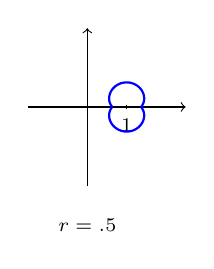
\begin{tikzpicture}[scale = .5]
    \node at (0,-3) {\begin{scriptsize}$r = .5$\end{scriptsize}}; 
    \draw [->, thin] (-1.5,0) -- (2.5,0);
    \draw [->, thin] (0,-2) -- (0,2);
    \draw (1, .05) -- (1, -.05) node [below] {\begin{scriptsize}$1$\end{scriptsize}};
    \draw [domain=0:2*pi, samples = 100, smooth, thick, blue]
      plot ({1 - 0.5*cos(\x r) + 0.125*cos(3*\x r)}, {-0.5*sin(\x r) + 0.125*sin(3*\x r)});
  \end{tikzpicture}
  \hfill
  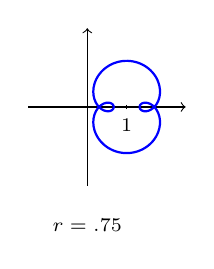
\begin{tikzpicture}[scale = .5]
    \node at (0,-3) {\begin{scriptsize}$r = .75$\end{scriptsize}}; 
    \draw [->, thin] (-1.5,0) -- (2.5,0);
    \draw [->, thin] (0,-2) -- (0,2);
    \draw (1, .05) -- (1, -.05) node [below] {\begin{scriptsize}$1$\end{scriptsize}};
    \draw [domain=0:2*pi, samples = 100, smooth, thick, blue]
      plot ({1 - 0.75*cos(\x r) + 0.421875*cos(3*\x r)}, {-0.75*sin(\x r) + 0.421875*sin(3*\x r)});
  \end{tikzpicture}
  \hfill
  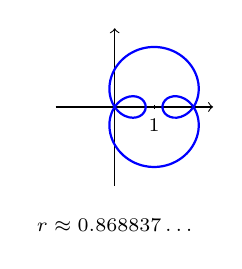
\begin{tikzpicture}[scale = .5]
    \node at (0,-3) {\begin{scriptsize}$r \approx 0.868837\dots$\end{scriptsize}}; 
    \draw [->, thin] (-1.5,0) -- (2.5,0);
    \draw [->, thin] (0,-2) -- (0,2);
    \draw (1, .05) -- (1, -.05) node [below] {\begin{scriptsize}$1$\end{scriptsize}};
    \draw [domain=0:2*pi, samples = 100, smooth, thick, blue]
    plot ({1 - 0.868837*cos(\x r) + 0.655866*cos(3*\x r)}, {-0.868837*sin(\x r) + 0.655866*sin(3*\x r)});
  \end{tikzpicture}

  \vfill 
\end{frame}


\begin{frame}
\frametitle{Common presentation mistakes}

\begin{columns}
\begin{column}{.65\textwidth}
\begin{itemize}
\item Too much content! \\[3ex]
\item Lots of text/math on a slide. \\[3ex]
\item Rapid speech without pauses. \\[3ex]
\item No images of cute puppies.  \\[3ex]
\item Lots of uncovering (a striptease).
\end{itemize}
\end{column}
\begin{column}{.35\textwidth}

\includegraphics[height=.66\textheight]{puppy.jpg}
\end{column}
\end{columns}
\end{frame}


\begin{frame}[fragile]
\frametitle{BibTeX can create a bibliography}

To print a \verb~.bib~ entry without \verb~\cite~ing, use \verb~\nocite~
\nocite{Manual, Metropolis, Themes}

\vfill

\bibliographystyle{plain} 
\bibliography{351Slides}

\vfill 

\end{frame}


\end{document}
